\documentclass{article}
% For math environments
\usepackage{amsmath, amsfonts}
% For links
\usepackage[colorlinks=true,
    linkcolor = blue,
    urlcolor  = blue,
    citecolor = blue,
    anchorcolor = blue]{hyperref}
% Put space between paragraphs
\usepackage{parskip}
% For figures
\usepackage{tikz}
% Set the margins to not be ridiculous
\usepackage[margin=0.75in]{geometry}
% For multiple columns
\usepackage{multicol}
% For controlling enum/itemize spacing and indentation
\usepackage{enumitem}
% More math symbols
\usepackage{amssymb}
% To change enumerate labels

% For tikz plots
\usepackage{pgfplots}
% This isn't needed but avoids a compiler warning
\pgfplotsset{compat=1.16}

% Allow multi-line equations to be broken across pages
\allowdisplaybreaks

% Use @ as a letter
\makeatletter

% Scale down all tikz coordinates while maintaining font size
\tikzset{every picture/.style={scale=0.45, every picture/.style={}}}


% Macros
% Monospace code
\def\code#1{\texttt{#1}}

% Greek letters
\def\a{\alpha}
\def\b{\beta}
\def\g{\gamma}
\def\d{\delta}
\def\D{\Delta}

% Commands that make life easier
\newcommand\gath[1]{\begin{gather} #1 \end{gather}}
\newcommand\ali[1]{\begin{align} #1 \end{align}}
\newcommand\parens[1]{\left( #1 \right)}
\newcommand\squares[1]{\left[ #1 \right]}
\newcommand\braces[1]{\left\{ #1 \right\}}
\newcommand\angles[1]{\left\langle #1 \right\rangle}
\newcommand\deriv[2]{\frac{d #1}{d #2}}
\newcommand\abs[1]{\left| #1 \right|}
\newcommand\floor[1]{\left\lfloor #1 \right\rfloor}
\DeclareMathOperator{\lcm}{lcm}
\def\non{\nonumber \\}

% Multiline equation space
\def\mlesp{\hspace{1.2cm}}

% For grid diagrams
\newcommand\gridbox[3]{\draw (#1,#2) rectangle (#1+1,#2+1) node[pos=.5] {#3};}
\newcommand\gridboxh[3]{\draw[fill=red!20] (#1,#2) rectangle (#1+1,#2+1) node[pos=.5] {#3};}
\newcommand\gridboxb[3]{\draw[fill=black] (#1,#2) rectangle (#1+1,#2+1) node[pos=.5] {#3};}
\newcommand\gridsym[3]{\node at (#1+0.5,#2+0.5) {$#3$};}
\newcommand\gridblank[2]{\filldraw[draw=gray, color=gray] (#1,#2) rectangle (#1+1,#2+1);}
\newcommand\gridcirc[2]{\draw (#1 + 0.5,#2 + 0.5) circle (0.25);}
\newcommand\cwlab[3]{
  \def\dd{0.15}
  \draw (#1 + \dd - 0.03, #2 + 1 - \dd) node {\scriptsize #3};
}

\def\bbw{3.5}
\def\bbh{2}
\newcommand\bigbox[3]{\draw (#1*\bbw,#2*\bbh) rectangle (#1*\bbw+\bbw,#2*\bbh+\bbh) node[pos=.5] {#3};}
\newcommand\bbtextr[3]{\node[right] at (#1*\bbw,#2*\bbh+0.5*\bbh) {#3};}
\newcommand\bbtextb[3]{\node[align=center] at (#1*\bbw+0.5*\bbw,#2*\bbh+0.5*\bbh) {#3};}

% Box puzzle stock answer
\newcommand\boxans[1]{
  Logic was used to deduce the solution:

  #1

  This was verified using Python as well as shown to be unique with a brute force approach.
}

% Multiple numbers
\newcommand\mn[1]{$#1$'s}

% Commands for problems
\newcommand\problem[4]{
  \section*{#1}

  Question: #3
  
  Answer: #2
  
  Explanation: #4
}
\newcommand\aproblem[4]{\problem{Dec #1}{#2}{#3}{#4}}
\newcommand\cproblem[4]{\problem{Problem #1}{#2}{#3}{#4}}

\def\advent@xxiv@i{
  Eve writes down five different positive integers.
  The sum of her integers is $16$. What is the product of her integers?
}

\def\advent@xxiv@ii{
  $14$ is the smallest even number that cannot be obtained by rolling two $6$-sided dice and finding the product of the numbers rolled.

  What is the smallest even number that cannot be obtained by rolling one hundred $100$-sided dice and finding the product of the numbers rolled?
}

\def\advent@xxiv@iii{
  There are $5$ ways to write $5$ as the sum of positive odd numbers:
  \begin{itemize}
    \item $1 + 1 + 1 + 1 + 1$
    \item $1 + 1 + 3$
    \item $3 + 1 + 1$
    \item $1 + 3 + 1$
    \item $5$
  \end{itemize}

  How many ways are there to write $14$ as the sum of positive odd numbers?
}

\def\advent@xxiv@iv{
  The geometric mean of a set of $n$ numbers is computed by mulitplying all the numbers together, then taking the $n$th root.
  The factors of $9$ are $1$, $3$, and $9$.
  The geometric mean of these factors is
  \gath{
    \sqrt[3]{1 \times 3 \times 9} = \sqrt[3]{27} = 3
  }
  What is the smallest number where the geometric mean of its factors is $13$?
}

\def\advent@xxiv@v{
  The sum of $11$ consecutive integers is $2024$.
  What is the smallest of the $11$ integers?
}

\def\advent@xxiv@vi{Put the digits 1 to 9 (using each digit exactly once) in the boxes so that the sums are correct. The sums should be read left to right and top to bottom ignoring the usual order of operations. For example, 4+3×2 is 14, not 10. Today's number is the product of the numbers in the red boxes.
  The number $n$ has $55$ digits.
  All of its digits are $9$.
  What is the sum of the digits of $n^3$?
}

\def\advent@xxiv@vii{
  What is the obtuse angle in degrees between the minute and hour hands of a clock at 08:22?
}

\def\advent@xxiv@viii{
  It is possible to arrange $4$ points on a plane and draw non-intersecting lines between them to form $3$ non-overlapping triangles:

  \begin{center}
    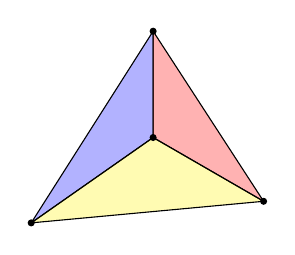
\begin{tikzpicture}
      \def\ds{3}
      \def\pa{(0: 0)}
      \def\pb{(90: \ds)}
      \def\pc{(215: 1.4*\ds)}
      \def\pd{(-30: 1.2*\ds)}

      \def\bcr{3}
      \def\scr{0.55*\bcr}
      \def\sca{34}
      \def\mcr{0.7*\bcr}
      \def\mca{142}
      \def\pr{0.1}

      % Triangles
      \draw[fill=blue,fill opacity=0.3] \pa -- \pb -- \pc -- cycle;
      \draw[fill=red,fill opacity=0.3] \pa -- \pb -- \pd -- cycle;
      \draw[fill=yellow,fill opacity=0.3] \pa -- \pd -- \pc -- cycle;

      % Points
      \fill \pa circle (\pr);
      \fill \pb circle (\pr);
      \fill \pc circle (\pr);
      \fill \pd circle (\pr);
    \end{tikzpicture}
  \end{center}

  It is not possible to make more than $3$ triangles with $4$ points.

  What is the maximum number of non-overlapping triangles that can be made by arranging $290$ points on a plane and drawing non-intersecting lines between them?
}

\def\advent@xxiv@ix{
  Put the digits $1$ to $9$ (using each digit exactly once) in the boxes so that the sums are correct.
  The sums should be read left to right and top to bottom ignoring the usual order of operations.
  For example, $4 + 3 \times 2$ is $14$, not $10$.
  Today's number is the product of the numbers in the red boxes.

  \grid@advent@xxiv@ix{}{}{}{}{}{}{}{}{}
}

\def\advent@xxiv@x{
  A number is a palindrome if it's the same when its digits are written in reverse order.

  What is the sum of all the numbers between $10$ and $100$ that are palindromes?
}

\def\advent@xxiv@xi{
  There are $6$ sets of integers between $1$ and $5$ (inclusive) that contain an odd number of numbers whose median value is $3$:

  \begin{itemize}
    \item $\braces{3}$
    \item $\braces{1,3,4}$
    \item $\braces{2,3,4}$
    \item $\braces{1,3,5}$
    \item $\braces{2,3,5}$
    \item $\braces{1,2,3,4,5}$
  \end{itemize}

  How many sets of integers between $1$ and $11$ (inclusive) are there that contain an odd number of numbers whose median value is $5$?
}

\def\advent@xxiv@xii{
  Holly picks a three-digit number.
  She then makes a two-digit number by removing one of the digits.
  The sum of her two numbers is $309$.
  What was Holly's original three-digit number?
}

\def\advent@xxiv@xiii{
  Today's number is given in this crossnumber.
  No number in the completed grid starts with $0$.

  \begin{multicols}{2}
    \crossnumstd{}{}{}{}{}{}{}{}{}

    \vfill\null
    \columnbreak

    \begin{center}
      \textbf{Across}

      \begin{tabular}{clc}
        \textbf{1} & Today's number.  & (\textbf{3}) \\
        \textbf{4} & Two times 5A.    & (\textbf{3}) \\
        \textbf{5} & A multiple of 1. & (\textbf{3})
      \end{tabular}

      \textbf{Down}

      \begin{tabular}{clc}
        \textbf{1} & Sum of digits is 15. & (\textbf{3}) \\
        \textbf{2} & Sum of digits is 19. & (\textbf{3}) \\
        \textbf{3} & Three times 5A.      & (\textbf{3})
      \end{tabular}
    \end{center}
  \end{multicols}
}

\def\advent@xxiv@xiv{
  $15^3$ is $3375$.
  The last $3$ digits of $15^3$ are $375$.

  What are the last $3$ digits of $15^{1234567890}$?
}

\def\advent@xxiv@xv{
  The number $2268$ is equal to the product of a square number (whose last digit is not $0$) and the same square number with its digits reversed: $36 \times 63$.

  What is the smallest three-digit number that is equal to the product of a square number (whose last digit is not $0$) and the same square number with its digits reversed?
}

\def\advent@xxiv@xvi{
  Put the digits $1$ to $9$ (using each digit exactly once) in the boxes so that the sums are correct.
  The sums should be read left to right and top to bottom ignoring the usual order of operations.
  For example, $4 + 3 \times 2$ is $14$, not $10$.
  Today's number is the product of the numbers in the red boxes.

  \grid@advent@xxiv@xvi{}{}{}{}{}{}{}{}{}
}

\def\advent@xxiv@xvii{
  The number $40$ has $8$ factors: $1$, $2$, $4$, $5$, $8$, $10$, $20$, and $40$.

  How many factors does the number $2^{26} \times 5 \times 7^5 \times 11^2$ have?
}

\def\advent@xxiv@xviii{
  TODO
}

\def\card@xxiv@i{
  What is the largest number you can make by using the digits $1$ to $4$ to make two $2$-digit numbers, then mutiplying the two numbers together?
}

\def\card@xxiv@ii{
  What is the largest number you can make by using the digits $0$ to $9$ to make a $2$-digit number and an $8$-digit number, then mutiplying the two numbers together?
}

\def\card@xxiv@iii{
  The expansion of $(2x+3)^2$ is $4x^2 + 12x + 9$.
  The sum of the coefficients of $4x^2 + 12x + 9$ is $25$.
  What is the sum of the coefficients of the expansion of $(30x + 5)^2$?
}

\def\card@xxiv@iv{
  What is the sum of the coefficients of the expansion of $(2x+1)^{11}$?
}

\def\card@xxiv@v{
  What is the geometric mean of all the factors of $41306329$?
}

\def\card@xxiv@vi{
  What is the largest number for which the geometric mean of all its factors is $92$?
}

\def\card@xxiv@vii{
  What is the sum of all the factors of $7^4$?
}

\def\card@xxiv@viii{
  How many numbers between $1$ and $28988500000$ have an odd number of factors?
}

\def\card@xxiv@ix{
  Eve found the total of the $365$ consecutive integers starting at $500$ and the total of the next $365$ consecutive integers, then subtracted the smaller total from the larger total.
  What was her result?
}

\def\card@xxiv@x{
  Eve found the total of the $n$ consecutive integers starting at a number and the total of the next $n$ consecutive integers, then subtracted the smaller total from the larger total.
  Her result was $22344529$.
  What is the largest possible value of $n$ that she could have used?
}

\input{boxes}

\begin{document}

\title{MS Scroggs Advent Calendar 2016 Answers}
\author{Dan Whitman}
\date{}

\maketitle

Answers: \href{https://www.mscroggs.co.uk/puzzles/advent2016}{https://www.mscroggs.co.uk/puzzles/advent2016}

\aproblem{1}{563}{\advent@xvi@i}{
  Suppose that today's number has the three digits $d_2 d_1 d_0$.
  If $d_2$ or $d_1$ were removed then the last digit of the sum would be $d_0 + d_0 = 2d_0$ and so would be even.
  As $9$ is odd, it means that $d_0$ must be the digit that was removed so that the two digit number therefore has digits $d_2 d_1$.
  Thus we have
  \begin{center}
    \begin{tabular}{c@{\,}c@{\,}c@{\,}c}
          & $d_2$ & $d_1$ & $d_0$ \\
      $+$ &       & $d_2$ & $d_1$ \\
      \hline
          & 6     & 1     & 9
    \end{tabular} \,.
  \end{center}
  Moreover, no digits can add to $19$ (since the biggest digit $9 + 9 = 18 < 19$) so that
  \gath{
    d_0 + d_1 = 9 \label{eqn:01:d0d1}
  }
  with no carry to the next digit.
  Since the middle digit of the sum is $1$, either $d_1 + d_2 = 1$ or $d_1 + d_2 = 11$.
  In the former case it has to be that $d_1 = 0$ and $d_2 = 1$ since otherwise the two digit number would actually only be a one digit number.
  However, in this case, it cannot possibly be that the first digit of the sum is $6$.
  So it must be that in fact
  \gath{
    d_1 + d_2 = 11 \label{eqn:01:d1d2}
  }
  so that $d_2 + 1 = 6$ because of the carry, and thus $d_2 = 6 - 1 = 5$.
  Hence $d_1 = 11 - d_2 = 11 - 5 = 6$ by \eqref{eqn:01:d1d2}, from which it follows from \eqref{eqn:01:d0d1} that $d_0 = 9 - d_1 = 9 - 6 = 3$.
  Therefore today's number is $d_2 d_1 d_0 = 563$.
}

\aproblem{2}{435}{\advent@xvi@ii}{
  If they are placed in an optimal way, each time a plane is added, it can intersect every already-placed plane.
  So clearly a single plane has $0$ intersections, adding a second plane adds $1$ intersection, adding a third plane adds $2$ more intersections, etc.
  Thus for $n$ planes the maximum number of intersecting lines is a triangular number:
  \gath{
    f(n) = \sum_{i=1}^{n-1} i = \frac{(n-1)(n-1 + 1)}{2} = \frac{n(n-1)}{2} \,.
  }
  Hence our answer is $f(30) = 435$.
}

\aproblem{3}{798}{\advent@xvi@iii}{
  Clearly the smallest such cube is such that the base of the pyramid is square and coincides with one side of the cube.
  The height of the pyramid then is also the same as the sides of the square base.
  If the sides of the enclosing cube have length $s$, then the base length, base width, and height of the pyramid are all $l = w = h = s$.
  The volume of the pyramid is then
  \gath{
    V_p = \frac{lwh}{3} = \frac{s^3}{3} \,.
  }
  The volume of the cube is of course simply
  \gath{
    V_c = s^3
  }
  so that $V_c = 3 V_p = 3 \cdot 266 = 798$, which is our answer.
}

\aproblem{4}{140}{\advent@xvi@iv}{
  \boxans{\gridsol@advent@xvi@iv}
}

\aproblem{5}{414}{\advent@xvi@v}{
  This was solved using Python.
}

\aproblem{6}{819}{\advent@xvi@vi}{
  Let $S(k)$ denote the digital sum of a non-negative integer $k$.
  We will prove the following set identity:
  \gath{
    \braces{S(k) \mid 1 \leq k \leq 10^n} = \braces{1, 2, \ldots, 9n}\,, \label{eqn:06:hyp}
  }
  for all integers $n \geq 1$.
  We show this by induction on $n$.
  In what follows define $A_n = \braces{S(k) \mid 1 \leq k \leq 10^n}$ and $B_n = \braces{1, 2, \ldots, 9n}$ so that we must show that $A_n = B_n$ for all $n \geq 1$.
  First, for $n = 1$, consider any $x \in A_n$ so that $x = S(k)$ for some $1 \leq k \leq 10^n = 10$.
  If $k$ is a single digit $1$ through $9$ then of course simply $x = S(k) = k$, and if $k = 10$ then of course $x = S(k) = 1$.
  Thus, in any case, $1 \leq x \leq 9 = 9n$ so that $x \in B_n$, and therefore $A_n \ss B_n$.
  Conversely, consider any $x \in B_n$ so that $1 \leq x \leq 9n = 9$ and simply set $k = x$ so that of course $x = S(k) = k$ since it is just a single digit.
  Since also clearly $1 \leq k = x \leq 9 \leq 10 = 10^n$, we have $x \in A_n$ so that $B_n \ss A_n$ as well.

  Now suppose that \eqref{eqn:06:hyp} is true for $n \geq 1$ and consider any $x \in A_{n+1}$ so that $x = S(k)$ for some $1 \leq k \leq 10^{n+1}$.
  If $k < 10^{n+1}$ then $k$ can be considered as an $n$-digit number where the first digit may be zero if $k < 10^n$.
  So let $d$ be the first digit and let $m$ be the integer formed by the remaining digits.
  Therefore $0 \leq d \leq 9$ and $m$ is a nonzero $(n-1)$-digit number and hence $1 \leq m < 10^n$.
  Thus $S(m) \in A_n = B_n$ by the induction hypothesis so that $1 \leq S(m) \leq 9n$.
  Since also clearly $x = S(k) = d + S(m)$, we have
  \gath{
    0 + 1 \leq d + S(m) \leq 9 + 9n \non
    1 \leq S(k) \leq 9(n+1) \non
    1 \leq x \leq 9(n+1)
  }
  so that $x \in B_{n+1}$, and hence $A_{n+1} \ss B_{n+1}$.
  Now suppose that $x \in B_{n+1}$ so that $1 \leq x \leq 9(n+1)$.
  In the case where $1 \leq x \leq 9n$ then $x \in B_n = A_n$ by the induction hypothesis, and so there is a $1 \leq k \leq 10^n$ where $x = S(k)$.
  Since also $1 \leq k \leq 10^n \leq 10^{n+1}$, it follows that $x = S(k) \in A_{n+1}$.
  In the other case where $9n < x \leq 9(n+1)$ set $d = 9$ and $y = x - d$ so that
  \gath{
    9n - 9 < x - 9 \leq 9(n+1) - 9 \non
    9(n-1) < x - d \leq 9n + 9 - 9 \non
    0 \leq 9(n-1) < x - d \leq 9n \non
    1 \leq y \leq 9n \,
  }
  noting that $0 \leq 9(n-1)$ since $1 \leq n$.
  Hence $y \in B_n = A_n$ by the induction hypothesis so that there is a $1 \leq k \leq 10^n$ such that $y = S(k)$.
  Now, if $k = 10^n$, then it must be that $y = S(k) = 1$, so let $m = k + 9 = 10^n + 9$ so that clearly
  \gath{
    1 + 9 \leq k + 9 \leq 10^n + 10 \non
    10 \leq k + 9 \leq 10^{n+1} \non
    1 \leq m \leq 10^{n+1} \,.
  }
  Since we also clearly have $x = y + d = y + 9 = 1 + 9 = 10 = S(10^n + 9) = S(m)$, it follows that $x \in A_{n+1}$.
  Otherwise we have $1 \leq k < 10^n$ so that $k$ is an $(n-1)$-digit number (where leading digits may be zero).
  So let $m$ be the number with leading digit $d = 9$ followed by the digits of $k$, resulting in an $n$-digit number so that $1 \leq m \leq 10^{n+1}$.
  Clearly also $S(m) = 9 + S(k) = 9 + y = d + y = x$.
  Thus we have that $x \in A_{n+1}$ and, as this is true in all cases, it follows that $B_{n+1} \ss A_{n+1}$, which completes the inductive proof of \eqref{eqn:06:hyp}.

  Clearly then our answer is $\abs{A_{91}} = \abs{B_{91}} = \abs{\braces{1, 2, \ldots, 9 \cdot 91}} = 9 \cdot 91 = 819$.
}

\aproblem{7}{691}{\advent@xvi@vii}{
  \boxans{\grid@advent@xvi@vii{3}{7}{5}{6}{9}{1}{4}{8}{2}}
}

\aproblem{8}{768}{\advent@xvi@viii}{
  Note that $a, b, \ldots, i$ are nine integers.
  Thus, the very smallest qualifying number would simply be $2^9 = 512$.
  The \emph{second}-smallest number is then simply changing \emph{one} of those \mn{2} to a $3$, that is $2^8 \cdot 3 = 768$.
}

\aproblem{9}{447}{\advent@xvi@ix}{
  This was solved using Python, as doing this potentially using the results of the 2015, Dec~9 would have been too complicated.
}

\aproblem{10}{171}{\advent@xvi@x}{
  We know that our solution $n$ has three digits.
  Let $s$ be the digital sum of $n$, which can can range from $1$, when $n = 100$, to $27$, when $n = 999$.
  For a given $s$, let $S(s)$ denote the digital sum of $s(s + 10)$ so that we must have $n = s(s + 10)$ and $s = S(s)$.
  Since we know the possible range of $s$, we can easily generate the following table:
  \begin{multicols}{3}
    \begin{center}
      \begin{tabular}{c|cc}
        $s$ & $n = s(s + 10)$ & $S(s)$ \\
        \hline
        1   & 11              & 2      \\
        2   & 24              & 6      \\
        3   & 39              & 12     \\
        4   & 56              & 11     \\
        5   & 75              & 12     \\
        6   & 96              & 15     \\
        7   & 119             & 11     \\
        8   & 144             & 9      \\
        9   & 171             & 9      \\
      \end{tabular}
    \end{center}
    \columnbreak

    \begin{center}
      \begin{tabular}{c|cc}
        $s$ & $n = s(s + 10)$ & $S(s)$ \\
        \hline
        10  & 200             & 2      \\
        11  & 231             & 6      \\
        12  & 264             & 12     \\
        13  & 299             & 20     \\
        14  & 336             & 12     \\
        15  & 375             & 15     \\
        16  & 416             & 11     \\
        17  & 459             & 18     \\
        18  & 504             & 9      \\
      \end{tabular}
    \end{center}
    \columnbreak

    \begin{center}
      \begin{tabular}{c|cc}
        $s$ & $n = s(s + 10)$ & $S(s)$ \\
        \hline
        19  & 551             & 11     \\
        20  & 600             & 6      \\
        21  & 651             & 12     \\
        22  & 704             & 11     \\
        23  & 759             & 21     \\
        24  & 816             & 15     \\
        25  & 875             & 20     \\
        26  & 936             & 18     \\
        27  & 999             & 27     \\
      \end{tabular}
    \end{center}
  \end{multicols}
  Inspecting the table, clearly $n \in \braces{171, 264, 375, 999}$ all have the defining property that $s = S(s)$.
  Of these, $n = 171$ is the smallest and is thus our answer.
}

\aproblem{11}{TODO}{\advent@xvi@xi}{
  TODO
}

\aproblem{12}{TODO}{\advent@xvi@xii}{
  TODO
}

\aproblem{13}{TODO}{\advent@xvi@xiii}{
  TODO
}

\aproblem{14}{TODO}{\advent@xvi@xiv}{
  TODO
}

\aproblem{15}{TODO}{\advent@xvi@xv}{
  TODO
}

\aproblem{16}{TODO}{\advent@xvi@xvi}{
  TODO
}

\aproblem{17}{TODO}{\advent@xvi@xvii}{
  TODO
}

\aproblem{18}{TODO}{\advent@xvi@xviii}{
  TODO
}

\aproblem{19}{TODO}{\advent@xvi@xix}{
  TODO
}

\aproblem{20}{TODO}{\advent@xvi@xx}{
  TODO
}

\aproblem{21}{TODO}{\advent@xvi@xxi}{
  TODO
}

\aproblem{22}{TODO}{\advent@xvi@xxii}{
  TODO
}

\aproblem{23}{TODO}{\advent@xvi@xxiii}{
  TODO
}

\aproblem{24}{TODO}{\advent@xvi@xxiv}{
  TODO
}

\end{document}
